\RequirePackage{lineno}
\documentclass[12pt]{article}
\usepackage[utf8]{inputenc}
\usepackage{fullpage}
\usepackage[T1]{fontenc}
\usepackage{amsmath, amsthm, amssymb,amsfonts}
\usepackage{mathptmx}
\usepackage{graphicx}

\usepackage{hyperref}
\hypersetup{colorlinks,
            citecolor=blue,
            filecolor=black,
            linkcolor=black,
            urlcolor=black
}

\title{Experimental overview of neutrino magnetic moment measurements}
\date{\today}

%\linenumbers % Include line numbers

\begin{document}
\maketitle

\section{Direct muon (anti)neutrino magnetic moment measurements}
\subsection{NOvA (Biao's thesis)}
\begin{itemize}
    \item $\nu_\mu$ only
    \item Only comparing total event counts - 25 events observed and 23.78 expected
    \item Put an upper limit ($90\%$ C.L.) of $\mu_{\nu_\mu}<1.58\times 10^{-9}\mu_B$ with $10.9\%$ systematic uncertainty on the standard model background
    \item Used $3.62\times 10^{20}$ POT of data ($6.74\times 10^{23}$ POT for MC) with $T\theta^2<0.003\textsf{GeV}\times\textsf{Rad}^2$, $0.3<T<0.9\textsf{GeV}$
\end{itemize}

\subsection{MiniBooNE}
\begin{itemize}
    \item $\nu_\mu$ only
    \item Observed excess of events (seems a bit too high)
\end{itemize}

\subsection{E734 at the Alternating Gradient Synchrotron (AGS) of the Brookhaven National Laboratory}
\begin{itemize}
    \item \textbf{Both $\nu_\mu$ and $\overline{\nu}_\mu$}
    \item $\mu_{\nu_\mu}<8.5\times 10^{-10}\mu_B$
%    \item \href{https://journals.aps.org/prd/abstract/10.1103/PhysRevD.41.3297}
\end{itemize}

\subsection{LSND}

\section{Direct electron (anti)neutrino magnetic moment measurements}

\section{Solar neutrino magnetic moment measurements}
\subsection{XENONnT}
First results published in arXiv:2207.11330\cite{XENON:2022mpc} on 22 July 2022.
\begin{itemize}
    \item 5.9 tonne dual-phase liquid xenon TPC dark matter detector
    \item Region Of Interest is (1,140)~keV
    \item Very low background (~5 times lower than XENON1T)
    \item Tritium excluded as the potential background (also in XENON1T)
    \item No excess found - XENON1T excess excluded with ~4$\sigma$
    \item The $90\%$ C.L. upper limit on solar neutrinos with an "enhanced" magnetic moment is \\$\mu_{\nu_{sol}}~<~6.3\times~10^{-12}\mu_B$, the strongest non-astronomical limit so far (see fig.\ref{fig:XENONnTResults})
\end{itemize}

\begin{figure}
    \centering
    \hspace*{1.5cm}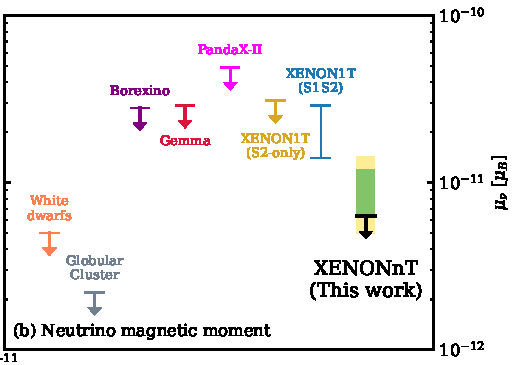
\includegraphics[width=.7\textwidth]{XENONnTExpResultsComparison.pdf}
    \caption{90\% C.L. upper limit on solar neutrinos with an enhanced magnetic moment.}
    \label{fig:XENONnTResults}
\end{figure}
Amir Khan used\cite{Khan:2022bel} XENONnT's results and derived limits on electromagnetic properties for the three SM neutrino flavours (see fig.\ref{fig:XENONnTFit_Khan}).
\begin{figure}
    \centering
    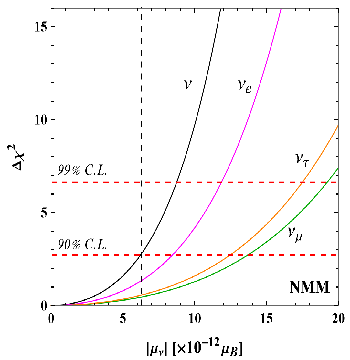
\includegraphics[width=.65\textwidth]{XENONnTFitForNuMM_Khan.pdf}
    \caption{One-dimensional $\Delta\chi^2$ distribution with 90\% and 99\% C.L. boundaries of neutrino magnetic moments. The distribution in black corresponds to the effective flavor independent magnetic moment}
    \label{fig:XENONnTFit_Khan}
\end{figure}
For $\nu_\mu$ they 

\subsection{XENON1T}

\subsection{BOREXINO}

\section{Other}
\subsection{LHC Forward Physics Facilities}
Preliminary sensitivity studies for future experiments (namely for FLArE and FASER$\nu$2)
\begin{itemize}
    \item LHC’s Forward Physics Facilities study high energy (TeV) neutrinos of all flavours from the ATLAS interaction point.
    \item Large opportunity to study tau neutrinos in more detail
\end{itemize}

\bibliographystyle{unsrturl}
\bibliography{ExperimentalOverviewNuMMLiterature}
\end{document}
